\documentclass[12pt,letterpaper]{article}
\usepackage[utf8]{inputenc}
\usepackage{listings, float, xcolor}

%----- Configuración del estilo del documento------%
\usepackage{graphicx, fancyhdr, lastpage}
\usepackage{enumitem, pifont, hyperref, ulem}
\usepackage[left=2cm,right=2cm,top=1.8cm,bottom=2.3cm]{geometry}

\pagestyle{fancy}
\fancyhf{}
\rfoot{\textit{Página \thepage \hspace{1pt} de \pageref{LastPage}}}

%------ Paquetes matemáticos básicos --------%
\usepackage{amsmath, amssymb, amsthm}

%------ Personalizar el link al video  --------%
\hypersetup{
  colorlinks=true,
  linkcolor=blue!50!black, % Azul oscuro
  urlcolor=blue!50!black,  % Azul oscuro
  hidelinks % Elimina el recuadro azul
}

\newcommand{\imp}{\rightarrow}

\begin{document}

%------ Encabezado -------- %
\begin{center}
  \begin{minipage}{3cm}
    \begin{center}
      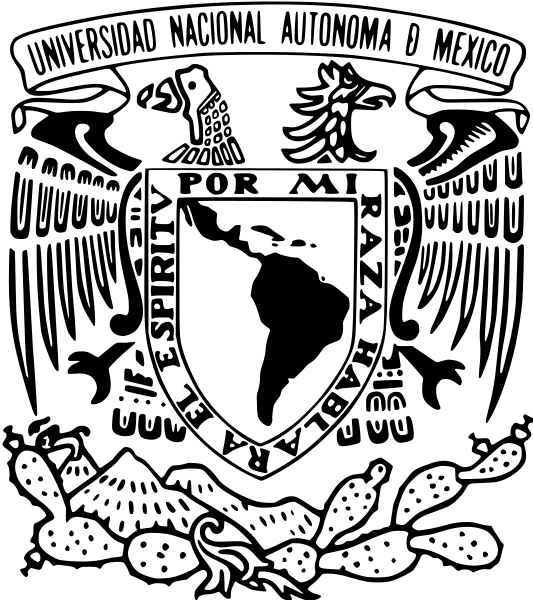
\includegraphics[height=3.4cm]{../unam_logo.png}
    \end{center}
  \end{minipage}\hfill
  \begin{minipage}{10cm}
    \begin{center}
      \textbf{\Large Universidad Nacional Autónoma de México}\\[0.2cm]
      \textbf{\large Facultad de Ciencias}\\[0.2cm]
      \textbf{Organización y Arquitectura de Computadoras 2025-2}\\[0.4cm]
      \textbf{\Large Tarea 02}\\[0.1cm]
      \textbf{Docentes:}\\
      José Galaviz \hspace{1em} Ricardo Pérez \hspace{1em} Ximena Lezama\\[0.3cm]
      \textbf{Autores:}\\
      Fernanda Ramírez Juárez \quad Ianluck Rojo Peña\\[0.2cm]
      \textbf{No. de cuenta:}\\
      321204747 \quad 118005762\\[0.2cm]
      \textbf{Fecha de entrega:} Jueves 27 de marzo de 2025
    \end{center}
  \end{minipage}\hfill
  \begin{minipage}{3cm}
    \begin{center}
      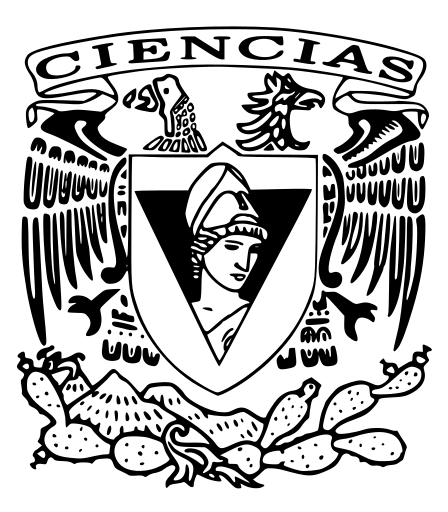
\includegraphics[height=3.4cm]{../fc_logo.png}
    \end{center}
  \end{minipage}
\end{center}

\bigskip
\hrule height 0.1pt
\bigskip

%------ Contenido -------- %
\section*{Preguntas.}

\begin{enumerate}
\item La Arquitectura de Computadoras se dedica únicamente al estudio de las instrucciones de una computadora y su desempeño respecto a estas ¿sí, no? Argumenta tu respuesta.
\bigskip
  % -- Respuesta -- %
  
\bigskip

\item ¿Los registros son dispositivos de hardware que permiten almacenar cualquier valor en binario? Argumenta tu respuesta.
  \bigskip
  % -- Respuesta -- %
  
  \bigskip
  
\item ¿Cuál es la diferencia entre un AMD Ryzen 5 y un Intel Core i5? ¿Qué tipo de organización de computadoras o microarquitectura tiene?
  \bigskip
  % -- Respuesta -- %
  
  \bigskip
  
\item De los dos tipos de arquitecturas, RISC y CISC. ¿Cuál de las dos requiere un mayor número de instrucciones para realizar una tarea? ¿Por qué crees que así sea?
  \bigskip
  % -- Respuesta -- %
  
  \bigskip

\item Menciona los tres factores de desempeño y de que dependen cada uno.
  \bigskip
  % -- Respuesta -- %
  
  \bigskip

\item Un programa tarda 9 millones de ciclos en una computadora cuyo ciclo dura 3 ns. ¿Cuál es el tiempo de CPU?
  \bigskip
  % -- Respuesta -- %
  
  \bigskip
  
\item Un programa tarda 14 millones de ciclos en una máquina a 2.4 GHz. ¿Cuál es el tiempo de CPU?
  \bigskip
  % -- Respuesta -- %
  
  \bigskip
  
\item ¿En una arquitectura CISC el periodo de una señal de reloj puede ser más grande que en una arquitectura RISC?
  \bigskip
  % -- Respuesta -- %
  
  \bigskip
  
\item El Intel 4004 (i4004), un CPU de 4 bits, fue el primer microprocesador en un simple chip, así como el primero disponible comercialmente y contenía 2300 transistores. Utilizando la Ley de Moore ¿Cuántos transistores se esperaría que tuviera hoy en día?
  \bigskip
  % -- Respuesta -- %
  
  \bigskip
  
\item El Intel Core i9-9900K es un procesador de 64 bits con 8 núcleos con tecnología Hyper-Threading de Intel, la cual ejecuta 2 hilos en cada núcleo por lo que cuenta con 16 hilos de procesamiento en total. El Intel Core i9-9900K cuenta con 3052 mil millones de transistores. Comparando con tu respuesta anterior ¿Es mayor o menor a lo esperado? ¿Se cumplió la ley de Moore? Argumenta tu respuesta.

  \bigskip
  % -- Respuesta -- %
  
  \bigskip
\end{enumerate}
\end{document}
